\subsection*{Общая характеристика работы}

% \newcommand{\actuality}{\underline{\textbf{Актуальность темы.}}}
% \newcommand{\aim}{\underline{\textbf{Целью}}}
% \newcommand{\tasks}{\underline{\textbf{задачи}}}
% \newcommand{\defpositions}{\underline{\textbf{Основные положения, выносимые на~защиту:}}}
% \newcommand{\novelty}{\underline{\textbf{Научная новизна:}}}
% \newcommand{\influence}{\underline{\textbf{Практическая значимость}}}
% \newcommand{\reliability}{\underline{\textbf{Достоверность}}}
% \newcommand{\probation}{\underline{\textbf{Апробация работы.}}}
% \newcommand{\contribution}{\underline{\textbf{Личный вклад.}}}
% \newcommand{\publications}{\underline{\textbf{Публикации.}}}
\newcommand{\actuality}{{\textbf{Актуальность темы.}}}
\newcommand{\aim}{{\textbf{Целью}}}
\newcommand{\tasks}{{\textbf{задачи}}}
\newcommand{\defpositions}{{\textbf{Основные положения, выносимые на~защиту:}}}
\newcommand{\novelty}{{\textbf{Научная новизна:}}}
\newcommand{\influence}{{\textbf{Практическая значимость}}}
\newcommand{\reliability}{{\textbf{Достоверность}}}
\newcommand{\probation}{{\textbf{Апробация работы.}}}
\newcommand{\contribution}{{\textbf{Личный вклад.}}}
\newcommand{\publications}{{\textbf{Публикации.}}}

%{\actuality} Эксперименты \belle и \babar, начавшие в $1999$ году набирать данные на $B$-фабриках \kekb и \pepii, соответственно, существенно продвинули понимание физики тяжелых кварков.  Ключевым результатом работы этих экспериментов стало наблюдение и детальное изучение нарушения \cpconj-симметрии в распадах $B$-мезонов.  Все обнаруженные \cpconj-нарушающие явления находятся в согласии с механизмом \cpconj-нарушения Кобаяши-Маскавы (\km) для слабых заряженных токов.

Нарушение \cpconj-симметрии важно не только с точки зрения описания взаимодействий элементарных частиц. Нарушение этой симметрии необходимо для описания бариогенеза и механизма формирования преобладания материи над антиматерией в видимой части Вселенной.  Есть основания полагать, что требуемая для описания бариогенеза степень нарушения \cpconj-симметрии не может быть обеспечена \km-механизмом, поэтому прецизионное измерение параметров этого механизма и поиск новых механизмов нарушения \cpconj-симметрии являются актуальными задачами экспериментальной физики высоких энергий.

Анализ многочастичных распадов является замечательным инструментом для измерения параметров \cpconj-нарушения и осцилляций нейтральных мезонов.  В некоторых случаях использование многочастичных распадов является необходимым условием для измерения величины параметра (а не установления факта отличия его величины от нуля).  Особенностью таких измерений является необходимость обладать информацией о не наблюдаемой непосредственно фазе амплитуды многочастичного распада.  Амплитуда распада не может быть получена из первых принципов из-за непертурбативных эффектов квантовой хромодинамики.  Эта проблема может быть решена с помощью построения феноменологической модели амплитуды распада и вычисления фазы с помощью этой модели.  
Такой подход, однако, неизбежно приводит к неустранимой и плохо контролируемой модельной неопределенности, которая может стать определяющей при выполнении прецизионных измерений в экспериментах~\lhcb и~\belleii.

Альтернативный подход, в котором среднее значение разности фаз амплитуд распадов \dn- и \dnbar-мезонов для определенной области фазового пространства извлекаются из эксперимента, не требует построения модели.  Этот подход может применяться в экспериментах \lhcb, \belleii, а также на Чарм-Тау-фабрике.

\aim\ данной работы является разработка и доказательство практической реализуемости модельно-независимого подхода к измерению параметров смешивания мезонов и параметров нарушения \cpconj-симметрии с использованием многочастичных распадов $D$- и $B$-мезонов.

Для~достижения поставленной цели необходимо было решить следующие {\tasks}:
\begin{enumerate}
  \item Исследовать влияние осцилляций и прямого нарушения \cpconj-симметрии в распадах $D$-мезонов на измеряемую величину \cpconj-нарушающего параметра \gphi модельно-независимо измеряемую в распадах \bdk, \dkpp.
  \item Разработать модельно-независимый метод получения параметров осцилляций и параметров нарушения \cpconj-симметрии в осцилляциях $D$-мезонов.
  \item Разработать модельно-независимый метод получения параметра \cpconj-нарушения \pphi в распадах \bdh, \dbkpp, $h^0\in\{\pin,\eta^{(\prime)},\omega\}$.
  \item Выполнить модельно-независимое измерение параметра \pphi в вышеупомянутом распаде, используя разработанный метод.
\end{enumerate}

\defpositions
%%% Согласно ГОСТ Р 7.0.11-2011:
%% 5.3.3 В заключении диссертации излагают итоги выполненного исследования, рекомендации, перспективы дальнейшей разработки темы.
%% 9.2.3 В заключении автореферата диссертации излагают итоги данного исследования, рекомендации и перспективы дальнейшей разработки темы.
\begin{enumerate}
  \item Изучено влияние осцилляций нейтральных $D$-мезонов на наблюдаемую величину параметра \gphi в модельно-независимом измерении в распадах \bdk, \dkpp и предложена процедура, при которой осцилляции $D$-мезонов смещают наблюдаемую величину не более, чем на~$0.2\grad$.
  \item Показано, что в предположении сохранения \cpconj-симметрии в распадах \dnkpp и при существующих экспериментальных ограничениях на величину этого нарушения, смещение наблюдаемой величины \gphi при модельно-независимом измерении в распадах \bdk, \dkpp, не превосходит $3\grad$.
  \item Показано, что модельно-независимое получение параметра \gphi в распадах \bdk, \dkpp возможно без предположения сохранения \cpconj-симметрии в распадах \dnkpp; при этом не наблюдается существенного снижения статистической чувствительности.
  \item Предложен метод модельно-независимого измерения параметров смешивания и \cpconj-нарушения в смешивании нейтральных $D$-мезонов в процессе $\ep\to \ddbar{}^{*}$ без измерения времени распада~$D$.
  \item Предложен метод модельно-независимого получения параметров смешивания и \cpconj-нарушения в смешивании нейтральных $D$-мезонов в процессе \dstpdpip, \dnkpp с измерением времени распада~$D$.
  \item Предложен метод модельно-независимого измерения \cpconj-нарушающей фазы \pphi в распадах \bdsth, \dbkpp; данный метод позволяет разрешить неопределенность, присущую измерению $2\pphi$ в переходах~\btoccs.
  \item Впервые выполнено модельно-независимое измерение фазы \pphi в распадах \bdsth, \dbkpp и получен результат $\pphi = 11.7\grad\pm7.8\grad\pm2.1\grad$, позволяющий разрешить неопределенность значения $2\pphi$ на уровне достоверности, превышающем $5$ стандартных отклонений.
  \item Подготовлен алгоритм для автоматического измерения характеристик модуля усилителя-формирователя калориметра \belleii, который был использован для проверки характеристик всех изготовленных модулей.
\end{enumerate}
% \begin{enumerate}
%   \item На основе анализа \ldots
%   \item Численные исследования показали, что \ldots
%   \item Математическое моделирование показало \ldots
%   \item Для выполнения поставленных задач был создан \ldots
% \end{enumerate}

\begin{enumerate}
  \item Изучено влияние осцилляций нейтральных $D$-мезонов на наблюдаемую величину параметра \gphi в модельно-независимом измерении в распадах \bdk, \dkpp и предложена процедура, при которой осцилляции $D$-мезонов смещают наблюдаемую величину не более, чем на~$0.2\grad$.
  \item Показано, что в предположении сохранения \cpconj-симметрии в распадах \dnkpp и при существующих экспериментальных ограничениях на величину этого нарушения, смещение наблюдаемой величины \gphi при модельно-независимом измерении в распадах \bdk, \dkpp, не превосходит $3\grad$.
  \item Показано, что модельно-независимое получение параметра \gphi в распадах \bdk, \dkpp возможно без предположения сохранения \cpconj-симметрии в распадах \dnkpp; при этом не наблюдается существенного снижения статистической чувствительности.
  \item Предложен метод модельно-независимого измерения параметров смешивания и \cpconj-нарушения в смешивании нейтральных $D$-мезонов в процессе $\ep\to \ddbar{}^{*}$ без измерения времени распада~$D$.
  \item Предложен метод модельно-независимого получения параметров смешивания и \cpconj-нарушения в смешивании нейтральных $D$-мезонов в процессе \dstpdpip, \dnkpp с измерением времени распада~$D$.
  \item Предложен метод модельно-независимого измерения \cpconj-нарушающей фазы \pphi в распадах \bdsth, \dbkpp; данный метод позволяет разрешить неопределенность, присущую измерению $2\pphi$ в переходах~\btoccs.
  \item Впервые выполнено модельно-независимое измерение фазы \pphi в распадах \bdsth, \dbkpp и получен результат $\pphi = 11.7\grad\pm7.8\grad\pm2.1\grad$, позволяющий разрешить неопределенность значения $2\pphi$ на уровне достоверности, превышающем $5$ стандартных отклонений.
  \item Подготовлен алгоритм для автоматического измерения характеристик модуля усилителя-формирователя калориметра \belleii, который был использован для проверки характеристик всех изготовленных модулей.
\end{enumerate}

\novelty\ впервые выполнено модельно-независимое измерение параметра \pphi в распадах \bdsth, \dbkpp; впервые предложены свободные от модельной неопределенности методы измерения параметров смешивания $D$-мезонов и \cpconj-нарушающего параметра \pphi с использованием многочастичных распадов нейтральных $D$-мезонов.

\influence: предложенный метод измерения параметра \pphi, а также результаты исследования процедуры модельно-независимого измерения параметра \gphi используются и будут использоваться при выполнении прецизионных измерений в экспериментах \babar, \belle, \belleii и \lhcb.  Предложенный метод измерения параметров осцилляций $D$-мезонов может быть использован при выполнении измерений в эксперименте \besiii и в будущих экспериментах на Чарм-Тау-фабрике.

\reliability\ полученных результатов обеспечивается публикацией основных результатов в рецензируемых журналах с высокой цитируемостью. Результаты измерения параметра \pphi находятся в согласии с предыдущим измерением в эксперименте \belle, а также с результатом измерения, выполненного группой \babar.

\probation\ Основные результаты работы докладывались~на научных семинарах в ИЯФ СО РАН и KEK (Цукуба, Япония).  Результаты измерения параметра \pphi были доложены на конференциях XIII Heavy Quarks and Leptons conference (HQL 2016) и 38th International Conference On High Energy Physics (ICHEP 2016).

\contribution\ Изложенные в работе результаты получены автором лично либо при его определяющем вкладе.

\ifthenelse{\equal{\thebibliosel}{0}}{% Встроенная реализация с загрузкой файла через движок bibtex8
    \publications\ Основные результаты по теме диссертации изложены в XX печатных изданиях, 
    X из которых изданы в журналах, рекомендованных ВАК, 
    X "--- в тезисах докладов.%
}{% Реализация пакетом biblatex через движок biber
%Сделана отдельная секция, чтобы не отображались в списке цитированных материалов
    \begin{refsection}%
        \printbibliography[heading=countauthornotvak, env=countauthornotvak, keyword=biblioauthornotvak, section=1]%
        \printbibliography[heading=countauthorvak, env=countauthorvak, keyword=biblioauthorvak, section=1]%
        \printbibliography[heading=countauthorconf, env=countauthorconf, keyword=biblioauthorconf, section=1]%
        \printbibliography[heading=countauthor, env=countauthor, keyword=biblioauthor, section=1]%
        \publications\ Основные результаты по теме диссертации изложены в \arabic{citeauthor} печатных изданиях\nocite{mixing,bdpv_cpv,belle_beta_binned_dalitz,testbench,belle_gamma_binned_dalitz}, 
        \arabic{citeauthorvak} из которых изданы в журналах, рекомендованных ВАК\nocite{mixing,bdpv_cpv,belle_beta_binned_dalitz,testbench,belle_gamma_binned_dalitz}. 
%        \arabic{citeauthorconf} "--- в тезисах докладов\nocite{confbib1,confbib2}.
    \end{refsection}
}


 % Характеристика работы по структуре во введении и в автореферате не отличается (ГОСТ Р 7.0.11, пункты 5.3.1 и 9.2.1), потому её загружаем из одного и того же внешнего файла, предварительно задав форму выделения некоторым параметрам

{\actuality} Эксперименты \belle и \babar, начавшие в $1999$ году набирать данные на $B$-фабриках \kekb и \pepii, соответственно, существенно продвинули понимание физики тяжелых кварков.  Ключевым результатом работы этих экспериментов стало наблюдение и детальное изучение нарушения \cpconj-симметрии в распадах $B$-мезонов.  Все обнаруженные \cpconj-нарушающие явления находятся в согласии с механизмом \cpconj-нарушения Кобаяши-Маскавы (\km) для слабых заряженных токов.

В некоторых случаях использование многочастичных распадов является необходимым условием для измерения величины параметра (а не установления факта отличия его величины от нуля).  Особенностью таких измерений является необходимость обладать информацией о не наблюдаемой непосредственно фазе амплитуды многочастичного распада.  Амплитуда распада не может быть получена из первых принципов из-за непертурбативных эффектов квантовой хромодинамики.  Эта проблема может быть решена с помощью построения феноменологической модели амплитуды распада и вычисления фазы с помощью этой модели.  
Такой подход, однако, неизбежно приводит к неустранимой и плохо контролируемой модельной неопределенности, которая может стать определяющей при выполнении прецизионных измерений в экспериментах~\lhcb и~\belleii.

Альтернативный подход, в котором среднее значение разности фаз амплитуд распадов \dn- и \dnbar-мезонов для определенной области фазового пространства извлекаются из эксперимента, не требует построения модели.  Этот подход может применяться в экспериментах \lhcb, \belleii, а также на Чарм-Тау-фабрике.

\aim\ данной работы является разработка и доказательство практической реализуемости модельно-независимого подхода к измерению параметров смешивания мезонов и параметров нарушения \cpconj-симметрии с использованием многочастичных распадов $D$- и $B$-мезонов.

Для~достижения поставленной цели необходимо было решить следующие {\tasks}:
\begin{enumerate}
  \item Исследовать влияние осцилляций и прямого нарушения \cpconj-симметрии в распадах $D$-мезонов на измеряемую величину \cpconj-нарушающего параметра \gphi модельно-независимо измеряемую в распадах \bdk, \dkpp.
  \item Разработать модельно-независимый метод получения параметров осцилляций и параметров нарушения \cpconj-симметрии в осцилляциях $D$-мезонов.
  \item Разработать модельно-независимый метод получения параметра \cpconj-нарушения \pphi в распадах \bdh, \dbkpp, $h^0\in\{\pin,\eta^{(\prime)},\omega\}$.
  \item Выполнить модельно-независимое измерение параметра \pphi в вышеупомянутом распаде, используя разработанный метод.
\end{enumerate}

\defpositions
%%% Согласно ГОСТ Р 7.0.11-2011:
%% 5.3.3 В заключении диссертации излагают итоги выполненного исследования, рекомендации, перспективы дальнейшей разработки темы.
%% 9.2.3 В заключении автореферата диссертации излагают итоги данного исследования, рекомендации и перспективы дальнейшей разработки темы.
\begin{enumerate}
  \item Изучено влияние осцилляций нейтральных $D$-мезонов на наблюдаемую величину параметра \gphi в модельно-независимом измерении в распадах \bdk, \dkpp и предложена процедура, при которой осцилляции $D$-мезонов смещают наблюдаемую величину не более, чем на~$0.2\grad$.
  \item Показано, что в предположении сохранения \cpconj-симметрии в распадах \dnkpp и при существующих экспериментальных ограничениях на величину этого нарушения, смещение наблюдаемой величины \gphi при модельно-независимом измерении в распадах \bdk, \dkpp, не превосходит $3\grad$.
  \item Показано, что модельно-независимое получение параметра \gphi в распадах \bdk, \dkpp возможно без предположения сохранения \cpconj-симметрии в распадах \dnkpp; при этом не наблюдается существенного снижения статистической чувствительности.
  \item Предложен метод модельно-независимого измерения параметров смешивания и \cpconj-нарушения в смешивании нейтральных $D$-мезонов в процессе $\ep\to \ddbar{}^{*}$ без измерения времени распада~$D$.
  \item Предложен метод модельно-независимого получения параметров смешивания и \cpconj-нарушения в смешивании нейтральных $D$-мезонов в процессе \dstpdpip, \dnkpp с измерением времени распада~$D$.
  \item Предложен метод модельно-независимого измерения \cpconj-нарушающей фазы \pphi в распадах \bdsth, \dbkpp; данный метод позволяет разрешить неопределенность, присущую измерению $2\pphi$ в переходах~\btoccs.
  \item Впервые выполнено модельно-независимое измерение фазы \pphi в распадах \bdsth, \dbkpp и получен результат $\pphi = 11.7\grad\pm7.8\grad\pm2.1\grad$, позволяющий разрешить неопределенность значения $2\pphi$ на уровне достоверности, превышающем $5$ стандартных отклонений.
  \item Подготовлен алгоритм для автоматического измерения характеристик модуля усилителя-формирователя калориметра \belleii, который был использован для проверки характеристик всех изготовленных модулей.
\end{enumerate}
% \begin{enumerate}
%   \item На основе анализа \ldots
%   \item Численные исследования показали, что \ldots
%   \item Математическое моделирование показало \ldots
%   \item Для выполнения поставленных задач был создан \ldots
% \end{enumerate}

\begin{enumerate}
  \item Изучено влияние осцилляций нейтральных $D$-мезонов на наблюдаемую величину параметра \gphi в модельно-независимом измерении в распадах \bdk, \dkpp и предложена процедура, при которой осцилляции $D$-мезонов смещают наблюдаемую величину не более, чем на~$0.2\grad$.
  \item Показано, что в предположении сохранения \cpconj-симметрии в распадах \dnkpp и при существующих экспериментальных ограничениях на величину этого нарушения, смещение наблюдаемой величины \gphi при модельно-независимом измерении в распадах \bdk, \dkpp, не превосходит $3\grad$.
  \item Показано, что модельно-независимое получение параметра \gphi в распадах \bdk, \dkpp возможно без предположения сохранения \cpconj-симметрии в распадах \dnkpp; при этом не наблюдается существенного снижения статистической чувствительности.
  \item Предложен метод модельно-независимого измерения параметров смешивания и \cpconj-нарушения в смешивании нейтральных $D$-мезонов в процессе $\ep\to \ddbar{}^{*}$ без измерения времени распада~$D$.
  \item Предложен метод модельно-независимого получения параметров смешивания и \cpconj-нарушения в смешивании нейтральных $D$-мезонов в процессе \dstpdpip, \dnkpp с измерением времени распада~$D$.
  \item Предложен метод модельно-независимого измерения \cpconj-нарушающей фазы \pphi в распадах \bdsth, \dbkpp; данный метод позволяет разрешить неопределенность, присущую измерению $2\pphi$ в переходах~\btoccs.
  \item Впервые выполнено модельно-независимое измерение фазы \pphi в распадах \bdsth, \dbkpp и получен результат $\pphi = 11.7\grad\pm7.8\grad\pm2.1\grad$, позволяющий разрешить неопределенность значения $2\pphi$ на уровне достоверности, превышающем $5$ стандартных отклонений.
  \item Подготовлен алгоритм для автоматического измерения характеристик модуля усилителя-формирователя калориметра \belleii, который был использован для проверки характеристик всех изготовленных модулей.
\end{enumerate}

\novelty\ впервые выполнено модельно-независимое измерение параметра \pphi в распадах \bdsth, \dbkpp; впервые предложены свободные от модельной неопределенности методы измерения параметров смешивания $D$-мезонов и \cpconj-нарушающего параметра \pphi с использованием многочастичных распадов нейтральных $D$-мезонов.

\influence: предложенный метод измерения параметра \pphi, а также результаты исследования процедуры модельно-независимого измерения параметра \gphi используются и будут использоваться при выполнении прецизионных измерений в экспериментах \babar, \belle, \belleii и \lhcb.  Предложенный метод измерения параметров осцилляций $D$-мезонов может быть использован при выполнении измерений в эксперименте \besiii и в будущих экспериментах на Чарм-Тау-фабрике.

\reliability\ полученных результатов обеспечивается публикацией основных результатов в рецензируемых журналах с высокой цитируемостью. Результаты измерения параметра \pphi находятся в согласии с предыдущим измерением в эксперименте \belle, а также с результатом измерения, выполненного группой \babar.

\probation\ Основные результаты работы докладывались~на научных семинарах в ИЯФ СО РАН и KEK (Цукуба, Япония).  Результаты измерения параметра \pphi были доложены на конференциях XIII Heavy Quarks and Leptons conference (HQL 2016) и 38th International Conference On High Energy Physics (ICHEP 2016).

\contribution\ Изложенные в работе результаты получены автором лично либо при его определяющем вкладе.

\ifthenelse{\equal{\thebibliosel}{0}}{% Встроенная реализация с загрузкой файла через движок bibtex8
    \publications\ Основные результаты по теме диссертации изложены в XX печатных изданиях, 
    X из которых изданы в журналах, рекомендованных ВАК, 
    X "--- в тезисах докладов.%
}{% Реализация пакетом biblatex через движок biber
%Сделана отдельная секция, чтобы не отображались в списке цитированных материалов
    \begin{refsection}%
        \printbibliography[heading=countauthornotvak, env=countauthornotvak, keyword=biblioauthornotvak, section=1]%
        \printbibliography[heading=countauthorvak, env=countauthorvak, keyword=biblioauthorvak, section=1]%
        \printbibliography[heading=countauthorconf, env=countauthorconf, keyword=biblioauthorconf, section=1]%
        \printbibliography[heading=countauthor, env=countauthor, keyword=biblioauthor, section=1]%
        \publications\ Основные результаты по теме диссертации изложены в \arabic{citeauthor} печатных изданиях\nocite{mixing,bdpv_cpv,belle_beta_binned_dalitz,testbench,belle_gamma_binned_dalitz}, 
        \arabic{citeauthorvak} из которых изданы в журналах, рекомендованных~ВАК\nocite{mixing,bdpv_cpv,belle_beta_binned_dalitz,testbench,belle_gamma_binned_dalitz}. 
%        \arabic{citeauthorconf} "--- в тезисах докладов\nocite{confbib1,confbib2}.
    \end{refsection}
}

{\textbf{Объем и структура работы.}} Диссертация состоит из~введения, четырех глав, заключения и пяти~приложений. Объем диссертации составляет $172$~страницы текста с~$59$~рисунками и~$19$~таблицами. Список литературы содержит $138$~наименований.

%%%%%%%%%%%%%%%%%%%%%%%%%%%%%%%%%%%%%%%%%%%%%%%%%%%%%%%%%%%%%%%%
%%%%%%%%%%%%%%%%%%%%%%%%%%%%%%%%%%%%%%%%%%%%%%%%%%%%%%%%%%%%%%%%
%%%%%%%%%%%%%%%%%%%%%%%%%%%%%%%%%%%%%%%%%%%%%%%%%%%%%%%%%%%%%%%%

\subsection*{Содержание работы}
Во {\textbf{введении}} обосновывается актуальность исследований, проводимых в рамках данной диссертационной работы, формулируется цель, ставятся задачи работы, сформулированы научная новизна и практическая значимость представляемой работы.

{\textbf{Первая глава}} посвящена рассмотрению основных феноменологических подходов к изучению нарушения \cpconj-симметрии в ускорительных экспериментах и описанию экспериментального статуса изучения нарушения \cpconj-симметрии.

%Несохранение \cpconj-четности (\cpconj-нарушение) в слабых взаимодействиях было обнаружено экспериментально в $1963$ году при изучении распадов $K_L^0$-мезонов.  Вскоре после этого Сахаров отметил, что \cpconj-нарушение является одним из необходимых условий формирования барионной асимметрии.  После этого Кобаяши и Маскава предложили механизм (\km-механизм), который в случае трех поколений кварков приводит к нарушению \cpconj-симметрии в слабых заряженных токов.  % Согласно \km-механизму, \cpconj-нарушающие эффекты во всей полноте проявляются в распадах $B$-мезонов, в которых задействованы кварки трех поколений.  Начавшие в $2003$ работу эксперименты \babar и \belle на $B$-фабриках \pepii (США) и \kekb (Япония), соответственно, позволили детально изучить многие \cpconj-нарушающие феномены в распадах $B$-мезонов и подтвердить справедливость \km-механизма.

В рамках Стандартной Модели (СМ) нарушение \cpconj-симметрии (\cpconj-нарушение) описывается механизмом Кобаяши-Маскавы (\km), согласно которому лагранжиан слабых заряженных токов описывает взаимодействие кварковых полей $q_u$ и $q_b^{\prime}$, где $q_u=\{u, c, t\}$ --- вектор полей верхних кварков, а $q_b^{\prime} = \{d^{\prime}, s^{\prime}, b^{\prime}\}$ --- вектор линейных комбинаций полей нижних кварков:
\begin{equation}\label{eq:ckm}
 \left(
 \begin{array}{c}
   d^{\prime} \\
   s^{\prime} \\
   b^{\prime} \\
  \end{array}
  \right)
  = \vckm
  \left(
  \begin{array}{c}
   d \\ s \\ b \\
  \end{array}
  \right)
  =
  \left(
  \begin{array}{ccc}
   V_{ud} & V_{us} & V_{ub} \\
   V_{cd} & V_{cs} & V_{cb} \\
   V_{td} & V_{ts} & V_{tb} \\
  \end{array}
  \right)\left(
  \begin{array}{c}
   d \\ s \\ b \\
  \end{array}
  \right),
\end{equation}
где $\vckm$ --- унитарная матрица смешивания кварков, называемая матрицей Кабиббо-Кобаяши-Маскавы (\ckm).  Матрица смешивания антикварков получается комплексным сопряжением матрицы~\vckm.  Взаимодействие кварков отличается от взаимодействия антикварков, если $\vckm^*\neq \vckm$.  Матрица~\vckm задается тремя углами Эйлера и фазой~$\delta$, которая является единственным параметром СМ, отвечающим за \cpconj-нарушение.

Экспериментальная проверка механизма \km сводится к измерению величин элементов и проверке условия унитарности матрицы~\ckm.  Наиболее подходящим для экспериментальной проверки является соотношение
\begin{equation}\label{eq:ut}
 \frac{V_{ud}V_{ub}^*}{V_{cd}V_{cb}^*}+\frac{V_{td}V_{tb}^*}{V_{cd}V_{cb}^*} + 1 = 0,
\end{equation}
которое можно представить в виде треугольника на комплексной плоскости (рисунок~\ref{fig:UT}), называемого Треугольником Унитарности (\ut). Величины углов~\ut выражаются через элементы матрицы~\ckm следующим образом:
\begin{equation}\label{eq:ut_angles}
 \aphi = \arg\lbr-\frac{V_{td}V^*_{tb}}{V_{ud}V^*_{ub}}\rbr,\quad
 \pphi = \arg\lbr-\frac{V_{cd}V^*_{cb}}{V_{td}V^*_{tb}}\rbr,\quad
 \gphi = \arg\lbr-\frac{V_{ud}V^*_{ub}}{V_{cd}V^*_{cb}}\rbr.
\end{equation}
%Измерение длин сторон и величин углов \ut является одной из главных задач физики тяжелых кварков.

\begin{figure}[h]
 \centering
  \includegraphics[width=0.5\textwidth]{UT}
   \caption{Геометрическое представление соотношения~\eqref{eq:ut}.}
  \label{fig:UT}
\end{figure}

Величины всех углов и сторон \ut можно определить из наблюдений. Получившаяся переопределенная система ограничений позволяет выполнить прецизионную проверку соотношений треугольника для \ut.  Анализ показывает, что при текущей точности измерения параметров \ut, составляющей в среднем $5\%$-$10\%$, значимых нарушений СМ не выявлено.  Таким образом, необходимо дальнейшее повышение точности измерений.

%, а значит и проверку \km-механизма.  Любое противоречие может свидетельствовать о проявлении эффектов Новой Физики (НФ).

%Анализ показывает, что при текущей точности измерения параметров \ut, составляющей в среднем $5\%$-$10\%$, значимых нарушений СМ не выявлено.  Таким образом, необходимо дальнейшее повышение точности измерений.  %Оценки потенциальных возможностей реализуемых в настоящее время экспериментов (\lhcb и \belleii) показывают, что в ближайшие $5$-$10$ лет возможно достижение точности $1\%$-$3\%$ в измерении основных параметров~\ut.

%%%%%%%%%%%%%%%%%%%%%%%%%%%%%%%%%%%%%%%%%%%%%%%%%%%%%%%%%%%%%%%%%%%
%%%%%%%%%%%%%%%%%%%%%%%%%%%%%%%%%%%%%%%%%%%%%%%%%%%%%%%%%%%%%%%%%%%
%%%%%%%%%%%%%%%%%%%%%%%%%%%%%%%%%%%%%%%%%%%%%%%%%%%%%%%%%%%%%%%%%%%

{\textbf{Вторая глава}} посвящена описанию модельно-независимого подхода к анализу многочастичных распадов.  В этой главе предложены программы исследований для симметричной Чарм-Тау-фабрики и асимметричной $B$-фабрики, а также для эксперимента \lhcb, основанные на этом подходе.  

% Рассмотрение многочастичных распадов зачастую позволяет преодолеть ограничения феноменологических подходов, основанных на анализе двухчастичных распадов $B$- и $D$-мезонов.  
% С другой стороны, использование многочастичных распадов приводит к сложностям, связанным с ограниченным знанием динамики распада.  Амплитуда многочастичного распада является (комплексной) функцией, определенной в фазовом пространстве конечного состояния.  В отличие от модуля, комплексная фаза амплитуды многочастичного распада не может быть измерена непосредственно.  Чаще всего информацию о комплексной фазе амплитуды многочастичного распада получают исходя из модельных предположений.  
% Такой подход нельзя считать удовлетворительным, поскольку он приводит к неустранимой и сложно оцениваемой неопределенности, связанной как со значением параметров модели, так и с обоснованностью применения той или иной модели.  В экспериментах с большой статистикой эти неопределенности могут стать доминирующим фактором, определяющим точность измерений.

Гири с соавторами предложили идею модельно-независимого получения угла~\gphi~\ut в распадах \bdk, \dkpp.  Предложение состоит в использовании среднего значения разности фаз $\deld$ амплитуд распадов $\ad\equiv\mca\lbr\dnkpp\rbr$ и $\adbar\equiv\mca\lbr\dbkpp\rbr$ для нескольких областей фазового пространства:%.  Введем параметры
% \begin{equation}\label{eq:ki}
%  \ki = \frac{\int\ddlzarea\left|\ad\right|^2 \ddlz}
%             {\int\limits_{\mcd}\left|\ad\right|^2 \ddlz},\quad
%  \kbi = \frac{\int\ddlzarea\left|\adbar\right|^2 \ddlz}
%             {\int\limits_{\mcd}\left|\adbar\right|^2 \ddlz},
% \end{equation}
% и
\begin{equation}\label{eq:csi}
  \zi \equiv \ci + i\si = 
            \frac{\int\ddlzarea
            \left|\ad\right|\left|\adbar\right|
            e^{i\deld}\,\ddlz}
            {\int\ddlzarea\left|\ad\right|^2 \ddlz 
             \int\ddlzarea\left|\adbar\right|^2 \ddlz}
            ,
\end{equation}
где индекс $i$ обозначает номер области фазового пространства, $\mcd$ обозначает полное фазовое пространство, $\mcd_i$ обозначает область фазового пространства, соответствующую номеру~$i$ и $m^2_{\pm}\equiv m^2\lbr\ks\pi^{\pm}\rbr$ обозначают квадраты масс пар частиц конечного состояния (переменные Далица).  Параметры \ci и \si близки по смыслу к среднему в $i$-й области значению $\cos\deld$ и $\sin\deld$, соответственно.  Кроме того, вводят параметры \ki и \kbi,  обозначающие вероятность попадания события в $i$-ю область при распаде \dn- и \dnbar-мезона, соответственно.  Для произвольного разбиения значения параметров \ki, \kbi, \ci и \si могут быть получены в когерентных распадах $\dn\dnbar$ на симметричном коллайдере, работающем вблизи резонанса \ppsi.

Предполагая отсутствие \cpconj-нарушения в распадах $D$-мезонов, т.е. используя соотношение $\ad\dvar\equiv\adbar\dvarinv$, можно оптимизировать способ разбиения диаграммы Далица распада \dnkpp: выбрать $2\mcn$ области симметрично относительно перестановки $\mpsq\leftrightarrow\mmsq$.  Номера областей $i$ при этом принимают значения от $-\mcn$ до $\mcn$, исключая $0$, такие, что инверсия знаков номеров областей $i\to -i$ соответствует перестановке $\mpsq\leftrightarrow\mmsq$. При таких договоренностях выполняются соотношения
\begin{equation}\label{eq:cp-conserv-relations}
 \zi \equiv Z^*_{-i}\quad (C_i\equiv C_{-i},\quad S_i\equiv -S_{-i}),\quad \kbi \equiv \kmi.
\end{equation}
Форму областей разумно выбрать так, чтобы получить максимальную статистическую чувствительность к измеряемым параметрам.  Хорошее приближение к оптимальному способу разбиения дает критерий
\begin{equation}\label{eq:uniph}
 \frac{2\pi\left(i-\frac{1}{2}\right)}{\mcn} < \deld\dvar < \frac{2\pi\left(i+\frac{1}{2}\right)}{\mcn}\quad
 \left(\textrm{для}\ \mpsq>\mmsq\ \textrm{и}\ i>0\right).
\end{equation}
Полученное таким способом разбиение называют \emph{равномерным по фазе}.  Критерий~\eqref{eq:uniph} может быть использован только на основе модельных соображений, поскольку функция $\deld\dvar$ неизвестна.  Такое использование модели, однако, не приводит к систематической ошибке измерения.

\begin{figure}[htb]
\begin{minipage}[b]{0.5\textwidth}
 \centering
  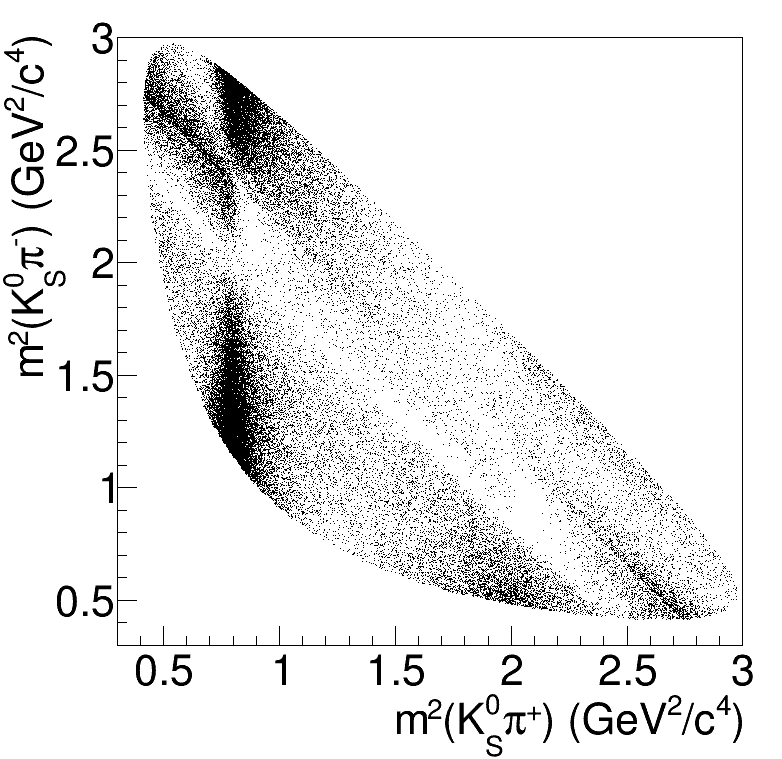
\includegraphics[width=0.85\textwidth]{dp_mc.png}
 \subcaption{}
 \label{fig:dalitz}
\end{minipage}
\begin{minipage}[b]{0.5\textwidth}
 \centering
  \includegraphics[width=0.9\textwidth]{belle_eqdel_bins}
 \subcaption{}
 \label{fig:bd_belle_eqph}
\end{minipage}
 \caption{а) Диаграмма Далица для распада \dbkpp и б)~равномерное по фазе разбиение этой диаграммы, выполненное с помощью модели, полученной с данными детектора \belle.}
 \label{fig:dalitz_plot}
\end{figure}

На рисунке~\ref{fig:dalitz_plot} показано распределение по переменным Далица (диаграмма Далица) для распада \dbkpp и равномерное по фазе разбиение, выполненное на основе полученной в эксперименте \belle модели.  

\paragraph{\boldmath Получение параметров смешивания в когерентных распадах $D$-мезонов.  }  Осцилляции $D$-мезонов описывают \emph{параметры смешивания}
\begin{equation}
 x_D \equiv \frac{\Delta m_D}{\Gamma_D},\quad y_D \equiv \frac{\Delta\Gamma_D}{2\Gamma_D},
\end{equation}
где $\Delta m_D$ ($\Delta\Gamma_D$) обозначает разность масс (ширин) массовых состояний нейтральных $D$-мезонов и $\Gamma_D$ обозначает полусумму ширин этих состояний.  Параметры смешивания малы $x_D\sim y_D\sim 10^{-2}$, поэтому мы всюду используем разложение в ряд по этим параметрам.

Параметры смешивания могут быть получены модельно-независимым образом в когерентных распадах пар $\dn\dnbar$, находящихся в симметричном по перестановке состоянии с $\cconj=+1$.\footnote{Для наглядности мы предполагаем сохранение \cpconj-симметрии в смешивании $D$-мезонов, хотя обсуждаемые ниже методы позволяют получить параметры \cpconj-нарушения в смешивании вместе с параметрами смешивания $D$-мезонов, если рассмотреть более общий формализм.}  Такие пары можно получить в распадах $\ep\to \dn\dbar{}^{*0}$, $\dbar{}^{*0}\to\dnbar\gamma$.  Пусть один из $D$-мезонов такой пары переходит в состояние~\kspp.  Вероятность попадания в область диаграммы Далица с индексом~$i$ при этом зависит от типа конечного состояния второго $D$-мезона.  При переходе второго $D$-мезона в \cpconj-собственное состояние с \cpconj-четностью~$\eta_D$ эта вероятность задается выражением
\begin{equation}\label{eq:m_cp_sym}
%  \begin{split}
   \left<M^{\cconj+}_{i,\eta_D}\right> 
   \propto \lbr\ki+\kmi\rbr\lbr1 + 2\eta_D y_D\rbr + 2\ci\sqrt{\ki\kmi}\lbr\eta_D + 2y_D\rbr %\\
   + \oxdydsq.
%  \end{split}
\end{equation}
Соответствующая вероятность при переходе второго $D$-мезона в состояние с определенным ароматом:
\begin{equation}\label{eq:m_flv_sym}
 \left<M^{\cconj+}_{i}\right> 
 \propto \ki + 2\sqrt{\ki\kmi}\lbr y_D\ci+x_D\si\rbr + \oxdydsq.
\end{equation}
Дополнительно можно рассмотреть некогерентный переход \dnbar-мезона, рожденного в процессе $\ep\to D^+D^{-*}$, $D^{-*}\to\dnbar\pi^+$, в состояние \kspp.  Вероятность попадания в область номер $i$ в этом случае:
\begin{equation}\label{eq:kprime}
 \ki^{\prime} \propto \ki + \sqrt{\ki\kmi}\lbr y_D\ci + x_D\si\rbr + \oxdydsq.
\end{equation}
При известных значениях параметров \ki, \ci и \si соотношения~\eqref{eq:m_cp_sym}, \eqref{eq:m_flv_sym} и~\eqref{eq:kprime} позволяют получить параметры смешивания $x_D$ и $y_D$.  

В процессе $\ep\to \dn\dbar{}^{*0}$, $\dbar{}^{*0}\to\dnbar\pin$ образуется когерентная пара~$\dn\dnbar$-мезонов в антисимметричном состоянии с $\cconj=-1$, которое позволяет получить не искаженные смешиванием значения параметров \ki, \ci и \si.  Таким образом, рассматривая совместно распады~$\dbar{}^{*0}\to\dnbar\pin$ и~$\dbar{}^{*0}\to\dnbar\gamma$, можно выполнить измерения, достаточные для получения параметров смешивания $D$-мезонов.  Оптимальной энергией коллайдера для предложенного измерения является~$4.01\gev$, которая находится под порогом рождения~$D^*\dbar{}^*$-пар.  Численные эксперименты показывают, что параметры смешивания могут быть получены с точностью около $10^{-3}$ с данными, соответствующими году работы Чарм-Тау-фабрики со светимостью~$10^{35}\lumi$.

\paragraph{\boldmath Получение параметров смешивания в некогерентных распадах $D$-мезонов с измерением времени распада. } Плотность вероятности перехода \dn-мезона, рожденного в процессе \dstpdpip, в состояние \kspp при условии попадания в $i$-ю область диаграммы Далица:
\begin{equation}\label{eq:kprime-time}
 \ki^{\prime}\lbr t\rbr \propto \dexp\left[ \ki+\sqrt{\ki\kmi}\lbr y_D\ci+x_D\si\rbr\Gamma t+ \oxdydtsq \right].
\end{equation}
%Большое количество нейтральных $D$-мезонов с известным ароматом в момент рождения позволяют получить распады \dstpdpip, в которых знак заряда $\pi$-мезона определяет начальный аромат $D$-мезона.  
Соотношение~\eqref{eq:kprime-time} впервые опубликовано в работе автора диссертации и позволяет получить параметры \ki и параметры смешивания $D$-мезонов во времязависимых измерениях на $B$-фабрике или в эксперименте~\lhcb.  Как уже обсуждалось, значения параметров~\ci и~\si могут быть получены независимо.  Первое получение параметров смешивания описанным методом было выполнено недавно группой~\lhcb. %В этом измерении использованы значения параметров~\ci и~\si, полученные в эксперименте~CLEO.  

\paragraph{\boldmath Влияние смешивания $D$-мезонов и прямого \cpconj-нарушения в распаде \dnkpp на получение угла \gphi. } В перспективе прецизионного модельно-независимого получения угла~\gphi в экспериментах~\belleii и~\lhcb важным вопросом является влияние осцилляций $D$-мезонов на величину~\gphi, полученную модельно-независимом способом в распадах \bdk, \dkpp.  Мы рассмотрели две процедуры: согласно первой процедуре для определения~\gphi используются значения параметров~\ki, \ci и~\si, полученные в когерентных распадах $\dn\dnbar$-пар; вторая процедура отличается от первой тем, что значения параметров~\ki получены в некогерентных распадах, и поэтому искаженны смешиванием (смотрите уравнение~\eqref{eq:kprime}).  %Смешивание $D$-мезонов в обоих процедурах не учитывается при определении величины \gphi.

Смещение \gphi для обоих процедур оценено с помощью численных экспериментов.  Первая процедура (\ki получены в когерентных распадах) приводит к смещению, не превышающему
\begin{equation}
 \delta\gphi^{(\mathrm{max})} = 3\grad\times \frac{\sqrt{x_D^2+y_D^2}}{0.1\rb}\approx 3\grad,\quad \rb = \left|\frac{\mca\lbr B^+\to\dn K^+\rbr}{\mca\lbr B^+\to\dnbar K^+\rbr}\right|.
\end{equation}
При использовании второй процедуры вклад смешивания в вероятность попадания события в область фазового пространства с индексом $i$ дополнительно подавлен фактором порядка \rb и максимальное смещение составляет
\begin{equation}
 \delta\gphi^{(\mathrm{max})} \approx 3\grad\times\rb\times \frac{\sqrt{x_D^2+y_D^2}}{0.1\rb}\approx 0.2\grad.
\end{equation}
Полученные результаты позволяют заключить, что получение параметров~\ki в некогерентных распадах позволяет не учитывать смешивание $D$-мезонов даже при прецизионном модельно-независимом получении~\gphi в эксперименте~\belleii (точность которого может быть близка к $1\grad$).  

%\paragraph{\boldmath Влияние прямого CP-нарушения в распадах D-мезонов на модельно-независимое получение параметра \gphi. } 
С помощью численных экспериментов изучено влияние прямого \cpconj-нарушения в распадах \dnkpp на извлекаемую модельно-независимым способом величину угла~\gphi в распадах~\bdk, \dkpp.  Показано, что смещение~\gphi не превосходит $3\grad$.  Эта величина определяется точностью экспериментального ограничения величины \cpconj-нарушения в распадах \dnkpp, полученного в эксперименте~CDF.  Ожидается, что измерения в экспериментах \lhcb и \belleii позволят значительно уменьшить эту величину, поскольку в СМ не ожидается значимых \cpconj-нарушающих эффектов в распадах $D$-мезонов.  
%Самое точное на данный момент ограничение величины \cpconj-нарушения в распадах \dnkpp получено в эксперименте CDF.  Используя этот результат, посредством численных экспериментом, показано, что смещение наблюдаемой величины угла \gphi при модельно-независимом измерении в распадах \bdk не превосходит $3\grad$.  

Кроме того, показано, что угол \gphi может быть извлечен в распадах \bdk, \dkpp модельно-независимо и без предположения сохранения \cpconj-симметрии в распадах \dnkpp. При этом статистическая чувствительность метода уменьшается незначительно.

\paragraph{\boldmath Модельно-независимое получение угла \pphi. }  Бондарь, Гершон и Кроковный предложили получать угол \pphi в распадах \bdsth, \dbkpp, $h\in\{\pin\eta^{(\prime)},\omega\}$.  Этот метод позволяет разрешить дискретную неопределенность $2\pphi\to\pi-2\pphi$, присущую классическому получению величины \sindbeta в кварковых переходах \btoccs.  Модельно-независимая модификация этого метода, предложенная автором диссертации, приводит к следующему выражению для плотности вероятности распада в~$i$-й области:
\begin{equation}\label{eq:master-formula}
 \begin{split}
  \mcp_i\lbr \dt\rbr &\propto \bexp\left[ 1 + q_B\frac{\ki-\kmi}{\ki+\kmi}\cos\dmdt\right.\\
  &\left.+2q_B\eta_{h^0}(-1)^l\frac{\sqrt{\ki\kmi}}{\ki+\kmi}\sin\dmdt\left(\si\cosdbeta+\ci\sindbeta\right)\right],
 \end{split}
 \end{equation} 
где $\dt$ обозначает разность собственных времен распада сигнального и помечающего $B$-мезонов, $q_B = 1$ ($q_B = -1$) соответствует аромату \bn (\bnbar) сигнального $B$-мезона при $\dt=0$, $\eta_{h^0}$ обозначает \cpconj-четность $h^0$-мезона и $l$ обозначает орбитальный момент $Dh^0$-системы.\footnote{Для распадов \bdstarh, \dbstdbpi, \dbkpp в функции \mcs возникает дополнительный множитель $-1$.}  

{\textbf{Третья глава}} посвящена описанию асимметричного электрон-позитронного ускорителя \kekb и детектора \belle.  В этой главе также обсуждается участие автора в модернизации калориметра детектора \belle для подготовки работы калориметра в эксперименте \belleii.  %Автором был разработан алгоритм измерения параметров 

В {\textbf{четвертой главе}} обсуждается выполненное впервые модельно-независимое измерение угла~\pphi в распадах \bdsth, \dbkpp, $h^0\in\{\pin, \eta, \etap, \omega\}$ (смотрите уравнение~\eqref{eq:master-formula}).  Для измерения использован полный интеграл светимости $711\ifb$, набранный детектором \belle вблизи резонанса \ups, соответствующий $771$ миллионам $\ups\to\bbbar$-событий.  Равномерное по фазе разбиение фазового пространства распада \dnkpp выполнено с помощью модели, полученной ранее в эксперименте~\belle.  Значения параметров \ci и \si для этого разбиения были измерены в эксперименте CLEO.  Значения параметров \ki получены с помощью распадов \bpdpi, \dbkpp.

Процедура анализа событий состоит из нескольких основных этапов.  На первом этапе происходит отбор кандидатов \bdsth с помощью различных кинематических параметров, изучение компонент фона и применение классифицирующих алгоритмов для подавления фона.  На втором этапе для каждого реконструируемого распада определяется доля сигнальных событий посредством анализа двумерного распределения параметров~\de и~\mbc:
\begin{equation}
 \de=E_B^{\cms}-E_{\mathrm{beam}}^{\cms},\quad
 \mbc = \sqrt{\left(E^{\cms}_{\mathrm{beam}}\right)^2-\left(p^{\cms}_{B}\right)^2},
\end{equation}
где $E_B^{\cms}$, $p^{\cms}_{B}$ и $E_{\mathrm{beam}}^{\cms}$ обозначают соответственно энергию $B$-кандидата, импульс $B$-кандидата и энергию пучка в системе центра масс.  Форма сигнального и фонового распределений \de-\mbc изучаются с помощью моделирования.  Заключительный этап анализа состоит анализе распределений по~\dt.  Фоновые \dt-распределения предварительно изучаются с помощью моделирования, а затем уточняются с помощью экспериментальных событий.  Корректность описания фоновых \dt-распределений и функции разрешения по \dt для сигнальных событий контролируется посредством измерения времени жизни \bn-мезона в распадах \bdsth, \dbkpp.  Получение \cpconj-нарушающих параметров осуществляется методом максимального правдоподобия с функцией правдоподобия вида
\begin{equation}\label{eq:lh}
 \mcl(\xi) = \prod\limits_{j=1}^{N}\left[\fsigj\psig\lbr\dtj,\xi\rbr+\lbr 1-\fsigj\rbr\pbkg\lbr\dtj\rbr\right],
\end{equation}
где $N$ обозначает количество отобранных событий, $\psig$ ($\pbkg$) обозначает плотность вероятности для сигнальных (фоновых) событий, $\fsigj$ обозначает вероятность того, что событие $j$ является сигнальным и $\xi\in\{\sindbeta, \cosdbeta, \pphi\}$.  Границы (асимметричных) доверительных интервалов $[\xi_{\mathrm{nl}},\xi_{\mathrm{nr}}]$, соответствующие $n$ стандартным отклонениям, определяются условием
\begin{equation}
 n^{2} = -2\log\lambda(\xi_{\mathrm{nl}}) = -2\log\lambda(\xi_{\mathrm{nr}}),
\end{equation}
где $\xi_{\mathrm{nl}}$ ($\xi_{\mathrm{nr}}$) обозначает левую (правую) границу интервала и $-2\log\lambda(\xi)$ обозначает логарифм отношения вероятностей 
\begin{equation}\label{eq:confidence_intervals}
 -2\log\lambda(\xi)=-2\log\mcl(\xi,\hat{\hat{\vecp}}) + 2\log\mcl(\hat{\xi},\hat{\vecp}).
\end{equation}
Здесь \vecp обозначает множество параметров за исключением~$\xi$, от которых зависит функция правдоподобия~$\mcl$, $\hat{\xi}$ и $\hat{\vecp}$ обозначают значения параметров, минимизирующее функцию правдоподобия, $\hat{\hat{\vecp}}$ обозначает значения параметров, минимизирующие функцию правдоподобия для текущего значения~$\xi$.  На рисунке~\ref{fig:lambda} показаны логарифмы отношения вероятностей для \cpconj-нарушающих параметров.  Следующие значения соответствуют одному стандартному отклонению:
 \begin{equation}\label{eq:final_results}
 \begin{split}
  \sindbeta &= 0.43     \pm 0.27\stat    \pm 0.08    \syst,\\
  \cosdbeta &= 1.06     \pm 0.33\stat^{+0.21}_{-0.15}\syst,\\
  \pphi     &= 11.7\grad\pm 7.8\grad\stat\pm 2.1\grad\syst.
 \end{split}
 \end{equation}

Величина $\sindbeta=0.691\pm0.017$, полученная в кварковых переходах \btoccs, определяет абсолютное значение \cosdbeta, которому соответствуют два значения угла $\pphi\in[0\grad; 180\grad)$.  Представленное в данной работе измерение исключает отрицательное значение \cosdbeta, соответствующее $\pphi = 68.1\grad$, на уровне $5.1$ стандартных отклонений и находится в согласии с положительным значением \cosdbeta, соответствующим значению $\pphi = 21.9\grad$ на уровне $1.3$ стандартных отклонений.  Таким образом, представленное измерение разрешает неопределенность в значении угла \pphi, присущую измерению параметра \sindbeta в переходах \btoccs.

\begin{figure}[htb]
 \begin{minipage}[b]{0.32\textwidth}
  \centering
  \includegraphics[width=\textwidth]{sin_minos_errors_v4}
  \subcaption{}
 \end{minipage}
 \begin{minipage}[b]{0.32\textwidth}
  \centering
  \includegraphics[width=\textwidth]{cos_minos_errors_v4}
  \subcaption{}
 \end{minipage}
 \begin{minipage}[b]{0.32\textwidth}
  \centering
  \includegraphics[width=\textwidth]{phi1_minos_errors_v4}
  \subcaption{}
 \end{minipage}
  \caption{Логарифмы отношений вероятностей~\eqref{eq:confidence_intervals} для а)~\sindbeta, б)~\cosdbeta и в)~\pphi. Квадраты (круги) показывают значения без учета (с учетом) систематических неопределенностей.  Пунктирные и непрерывные линии показывают аппроксимацию полученных значений.  Вертикальные линии показывают значения, соответствующие $\sindbeta=0.691$.  }
  \label{fig:lambda}
\end{figure}

Доминирующие систематические неопределенности представленного измерения имеют статистическую природу.  Основной вклад вносит неопределенность значений параметров~\ci и~\si, полученных в эксперименте~CLEO.  Эти неопределенности могут быть уменьшены с помощью измерений в эксперименте~\besiii.  Другие существенные неопределенности связаны с описанием временного разрешения и распределений по параметрам~\de и~\mbc.  Эти неопределенности зависят от статистики и будут меньше при выполнении измерения в эксперименте~\belleii.  При выполнении описанного анализа, таким образом, показано отсутствие систематических неопределенностей, потенциально ограничивающих точность прецизионного измерения в эксперименте~\belleii.

В {\textbf{заключении}} приведены основные результаты работы и кратко описаны перспективы развития и практической реализации предложенных в работе методов модельно-независимого получения параметров в экспериментах \belleii, \lhcb и на Чарм-Тау-фабрике.


%\newpage
%При использовании пакета \verb!biblatex! список публикаций автора по теме
%диссертации формируется в разделе <<\publications>>\ файла
%\verb!../common/characteristic.tex!  при помощи команды \verb!\nocite! 

%\clearpage
\ifthenelse{\equal{\thebibliosel}{0}}{% Встроенная реализация с загрузкой файла через движок bibtex8
  \renewcommand{\refname}{\large \authorbibtitle}
  \nocite{*}
  \insertbiblioauthor                          % Подключаем Bib-базы
  %\insertbiblioother   % !!! bibtex не умеет работать с несколькими библиографиями !!!
}{% Реализация пакетом biblatex через движок biber
  \insertbiblioauthor                          % Подключаем Bib-базы
%  \insertbiblioother
}

